\documentclass{article}[12 pt]

% Multiline equations
\usepackage{amsmath}

% Make margins bigger
\usepackage{geometry}
\geometry{
	a4paper,
}

% Change the language for the captions and default names
\renewcommand{\figurename}{Figura}

% Change the language for the table of contens
\renewcommand{\contentsname}{Contenidos}

% Insert images
\usepackage{graphicx}
% Look for images here
\graphicspath{{Img/}}

\title{Diseñando la ICT de un chalet\thanks{Proudly made with \LaTeX}}
\author{Carlos Ortega Marchamalo \& Pablo Collado Soto \\ \\ \textbf{\texttt{Sistemas Inteligentes y Sostenibles de Nueva Generación}} \\ \\ \textbf{Universidad de Alcalá}}
\date{}

\begin{document}
	\maketitle

	\newpage

	\tableofcontents

	\newpage

	\section{Introducción}
		Antes de inventar una vivienda para posteriormente diseñar su Infraestructura Común de Telecomunicación o de escoger una ICT ya diseñada para analizarla hemos decidido estudiar una instalación real. La ICT a la que nos atendremos durante el informe pertenece a una vivienda unifamiliar de la Urbanización Sotolargo en la Provincia de Guadalajara. Hemos optado por estudiar la ICT de un chalet en vez de la de un bloque de edificios para profundizar en este tipo de inmueble ya que es el que menos hemos estudiado en las clases teóricas de la asignatura. Asimismo, esto nos permite acercarnos a una situación real que en ocasiones queda muy lejos de las aulas. Con ello esperamos ser capaces de tener en cuenta las limitaciones que nos impiden aplicar directamente la teoría al mundo real.\\

		Además de estudiar la \textbf{ICT} propiamente dicha hemos decidido también abordar la red telefónica y de datos. Al situarse el inmueble en una zona alejada de grandes ciudades veremos que el acceso es todavía a través de una línea ADSL (\textbf{A}bonado \textbf{Digital} \textbf{A}simétrico) por lo que lo compararemos con los accesos actuales basados en su mayoría en fibra óptica.\\

		Las frecuencias analizadas se encuentran en la región \textbf{UHF} (\textbf{U}ltra \textbf{H}igh \textbf{F}requencies) ya que nos centraremos en la infraestructura de \textbf{T}elevisión \textbf{D}igital \textbf{T}errestre. Esta región se compone a su vez de las bandas \textit{BIV} y \textit{BV} que comprenden los rangos de frecuencia $[470, 606]\ MHz$ y $[606, 862]\ MHz$ respectivamente. A fin de no alargar el informe de manera innecesaria señalamos que todas las atenuaciones y características de los equipos analizados se ciñen a esta banda.\\

	\section{Fuentes de información}
		Con la intención de ajustarnos en la medida de lo posible a la realidad hemos consultado los planos de obra de la vivienda. No obstante hemos encontrado que, si bien se aludía a la \textbf{ICT} no se incluían detalles sobre la misma. Tan solo se señalaba la localización de una serie de tomas de televisión y teléfono sin mostrar las canalizaciones hasta las mismas. También encontramos que estos planos de obra no estaban actulizados pues las tomas físicas no se encontraban en los lugares señalados por los planos.\\

		Debido a esto, y tras consultar con el arquitecto de la vivienda nos decidimos a investigar la localización del registro primario para intentar reconstruir la \textbf{ICT} a partir de los equipos y líneas de transmisión instaladas. Asimismo, a la hora de calcular las atenuaciones en los cables hemos aproximado las distancias a partir de la planta acotada que se incluía en los planos de la vivienda. A pesar de que esto aporta una mayor fidelidad a los resultados debemos reconocer que no se ajustan de manera totalmente estricta a la realidad. Al observar los equipos instalados hemos visto que las líneas de transmisión discurren por el interior de los distintos tabiques, suelos y paredes con lo que deberemos tolerar esta pequeña inexactitud.

	\section{Equipamiento}
		Con tan solo retirar una cubierta de PVC hemos tenido acceso al registro primario del inmueble. Dentro hemos encontrado el siguiente equipo:

		\vskip 3mm

		\begin{center}
			\begin{tabular}{| c | c | c |}
				\hline
				\textbf{Equipo} & \textbf{Fabricante} & \textbf{Referencia}\\
				\hline
				Fuente de alimentación con 2 salidas & Televés & 5495\\
				\hline
				PAU/Repartidor & Televés & 5436\\
				\hline
				Punto de Terminación de Red & Telefónica & No Disponible\\
				\hline
				Cable Coaxial T-100 Plus & Televés & 2141\\
				\hline
				Cable Cobre CTX Cu & Televés & 2138\\
				\hline
				Tomas TV-RF/SAT* & Televés & 5226\\
				\hline
			\end{tabular}
		\end{center}

		\vskip 3mm

		Señalamos que las tomas TV-RF/SAT \textbf{NO} se encuentran en este registro primario pero hemos decidido incluirlas dada su estrecha relación con el resto de los aparatos. Asimismo, las referencias se pueden encontrar impresas sobre los equipos como por ejemplo en el cable coaxial que sale hacia la antena tal y como vemos en la figura \ref{f:coax}. Podemos observar la apariencia real de todos estos elementos en la imagen \ref{f:reg_primario} quedando las tomas reflejadas en la figura \ref{f:toma}.

		\begin{figure}
				\centering
				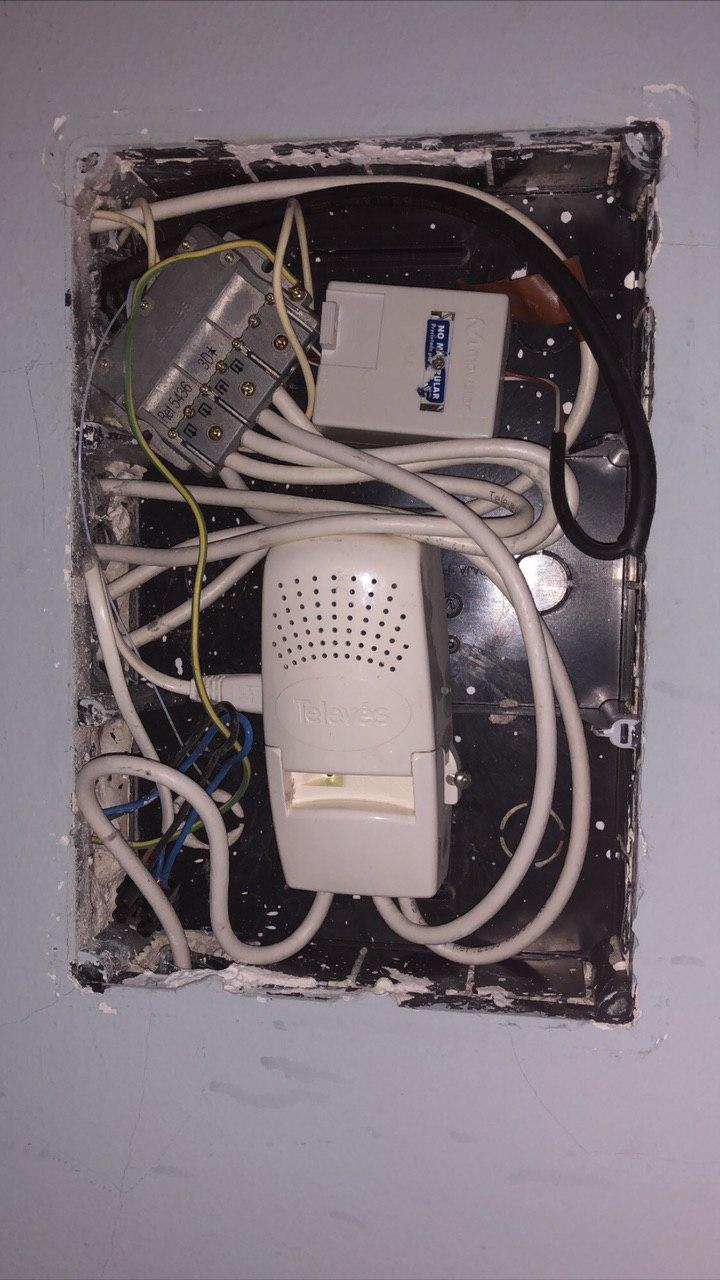
\includegraphics[scale=0.32, angle=90]{registro_primario.jpg}
				\caption{El registro primario}
				\label{f:reg_primario}
		\end{figure}

		\begin{figure}
				\centering
				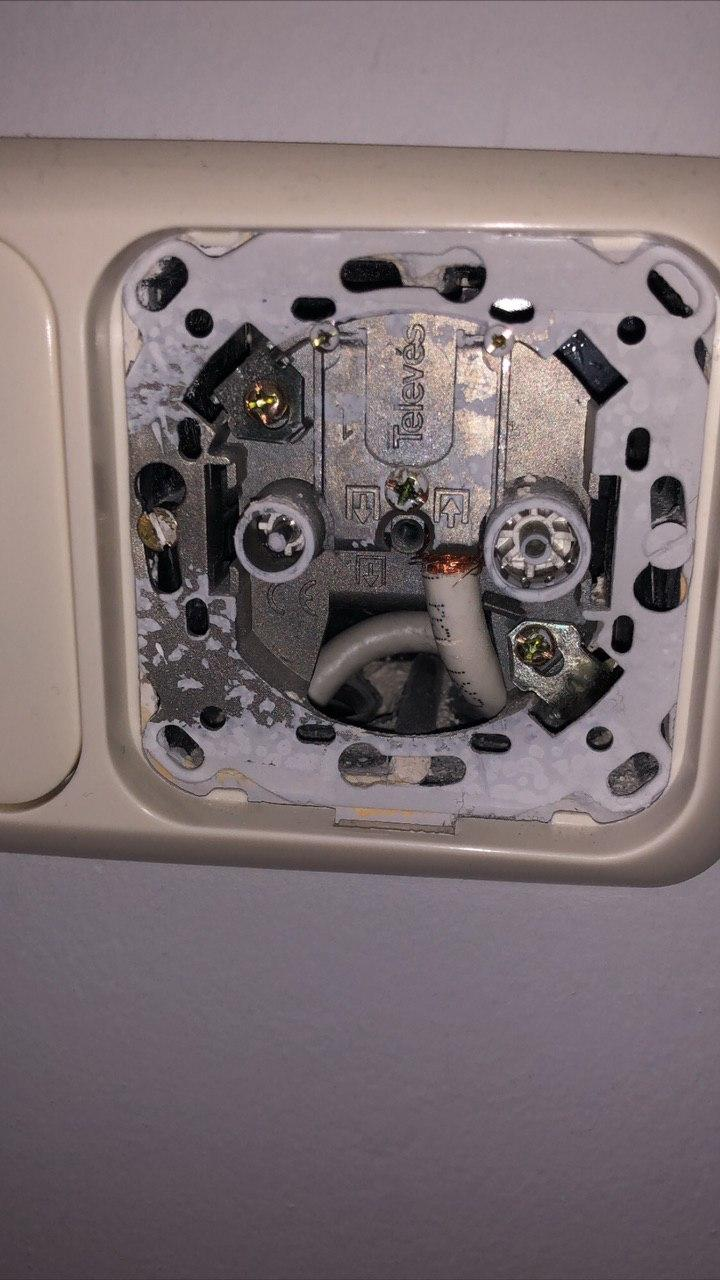
\includegraphics[scale=0.2]{enchufe_tv.jpg}
				\caption{Toma de TV y Satélite}
				\label{f:toma}
		\end{figure}

		Entre el equipo observado encontramos 2 elementos que \textit{a priori} nos resultan extraños. En primer lugar encontramos una fuente de alimentación. Si pensamos en la estructura de la ICT nos daremos cuenta de que la señal es captada por una antena diseñada para la banda de televisión y que esta deberá ser amplificada dada su amplitud tan reducida. Si modeláramos el circuito esta antena sería nuestro generador y la carga equivalente vendría a representar tanto las líneas de distribución como las cargas de los equipos conectados a las mismas.\\

		\begin{figure}
				\centering
				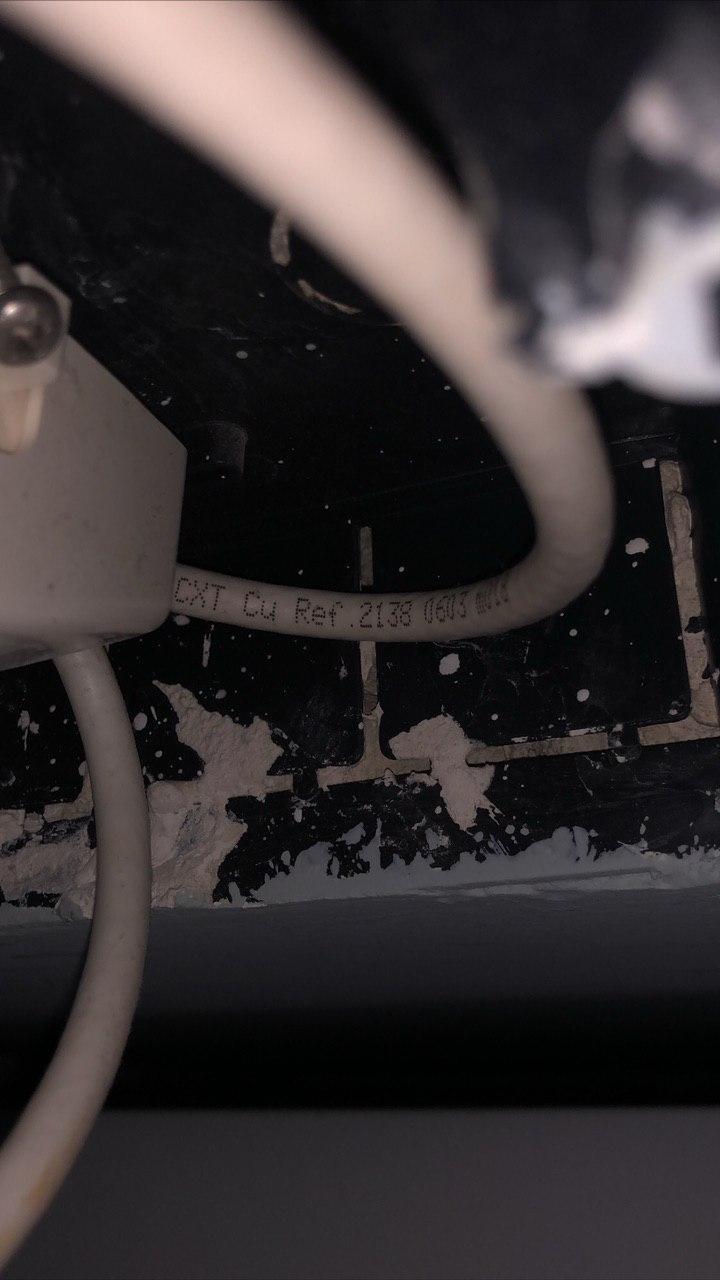
\includegraphics[scale=0.2, angle=90]{cable_cobre.jpg}
				\caption{Cable de cabecera}
				\label{f:coax}
		\end{figure}

		El hecho de que la señal de entrada a la \textbf{ICT} sea tan pequeña nos lleva a preguntarnos por qué no hemos incluido un amplificador en la tabla anterior. Destacamos pues que este amplificador de cabecera no se encuentra en el registro primario sino más cerca de la antena. Es por ello que no hemos tenido acceso al equipo en cuestión pero tras indagar llegamos a una configuración de equipos de Televés muy común en viviendas de este tipo que podemos ver en la figura \ref{f:schematic}. En ellas se incluye, como no podría ser de otra manera, un amplificador de cabecera con referencia \textbf{XXX}. Pasamos a hacer un pequeño inciso sobre el cálculo de ganancias y su uso a la hora de obtener las atenuaciones en la infraestructura analizada\\

		Además de todo este equipo dedicado a la infraestructura de \textbf{TDT} (exceptuando el \textit{Punto de Terminación de Red}) también encontramos elementos que juntos integran la red de datos y telefonía. Los incluimos en la siguiente tabla.

		\vskip 3mm

		\begin{center}
			\begin{tabular}{| c | c |}
				\hline
				\textbf{Equipo} & \textbf{Fabricante}\\
				\hline
				Splitter & Telefónica\\
				\hline
				Router/Módem & Telefónica\\
				\hline
			\end{tabular}
		\end{center}

		\vskip 3mm


		\begin{figure}
				\centering
				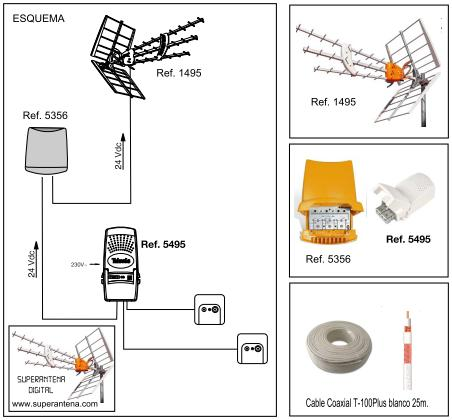
\includegraphics{schematic.jpg}
				\caption{Estructura general del sistema}
				\label{f:schematic}
		\end{figure}

		\subsection{Frecuencias, ganancias y $decibelios$}
			Los amplificadores son por definición circuitos activos (contienen elementos activos como transistores) ya que nos permiten manejar ganancias mayores que la unidad. Recordemos la definición de ganancia de un circuito:

			$$Sean\ v_i, v_o\ tensiones \rightarrow G = \frac{v_o}{v_i}$$

			Esto es, la ganancia es la relación entre las señales de entrada a un circuito y su salida. En este caso $v_i$ sería la señal de entrada al amplificador y $v_o$ la señal a la salida. De lo anterior se sigue que $G$ es un valor adimensional que caracteriza el amplificador utilizado. A pesar de lo aquí comentado debemos señalar que las señales $v_x$ son en general funciones del tiempo ($v(t)$) con lo que llevan asociado un espectro $V(w) = \mathcal{F}\{v(t)\}$ lo que supone una variación de esta ganancia con la frecuencia de las señales que manejos. Esto se resume estableciendo que $G \neq\ cte$ sino que es una función de la frecuencia $G(w)$.\\

			Dada esta variabilidad de la ganancia los fabricantes acompañan sus productos de un ancho de banda de trabajo para sus aparatos. Esto es una banda de frecuencias para las que se puede asumir que $G =\ cte$. Estas ganancias son las que nosotros veremos en las hojas del fabricante, en este caso Televés, cuando analicemos la ICT.\\

			No obstante al acudir a las hojas de características de los equipos nos percataremos de que la unidad de esta ganancia son $dB$, es decir, decibelios. A pesar de toda la confusión que estas generan (por lo menos a nosotros) las unidades logarítmicas están pensadas para facilitar el manejo de cantidades grandes. Dado que el $Belio$ es una unidad demasiado grande comúnmente trabajaremos con el $decibelio$. Al igual que con otras unidades se cumple que $1\ Belio =\ 10\ decibelios$. Con todo, las ganancias que podemos esperar son del tipo:

			$$G(dB) = 10 \cdot log(\frac{V_o}{V_i})$$

			Nos damos cuenta en un principio de que los decibelios son en realidad adimensionales al igual que otras unidades como los $radianes$. Al final estamos comparando dos magnitudes. Además, dadas las propiedades de los logaritmos veremos que en vez de multiplicar por las ganancias podemos sumar tensiones y decibelios siempre que las tensiones también estén expresadas en unidades logarítmicas. Esto se sigue de la definición misma de la ganancia que hemos visto anteriormente:

			$$G(dB) = 10 \cdot log(\frac{V_o}{1\ V}) - 10 \cdot log(\frac{V_i}{1\ V}) \rightarrow G(dB) = V_o(dBV) - V_i(dBV)$$

			Así llegamos a que $V_o(dBV) = G(dB) + V_i(dBV)$. Con este pequeño desarrollo explicamos el por qué de los cálculos que iremos haciendo a lo largo del informe. No debemos olvidar que podemos modelar cualquier línea de transmisión como los cables coaxiales de nuestra instalación como si se tratara de una "caja negra" con una relación de transmisión $\frac{V_o}{V_i}$ idéntica a la de este caso. Es por ello que si entendemos las atenuaciones como ganancias negativas el procedimiento para calcular todas las pérdidas de señal a lo largo de la instalación es análogo a este. Esperamos haber disipado las dudas que podríamos tener sobre la forma de operar con estas unidades que pueden jugarnos una mala pasada si no tenemos cuidado...\\

		\subsection{¿Qué son esos equipos?}
			Si queríamos dejar algo claro es que elementos activos como los amplificadores necesitan un lugar del que sacar la potencia que "inyectan" en su salida. Esto es, necesitamos alimentarlos. Es aquí donde se encuadra la fuente de alimentación que incluíamos en la relación de equipos. Este aparato se encargará de suministrar la alimentación (una tensión continua) requerida por el amplificador y por la antena. Además tal y como vemos en la figura \ref{f:schematic} se va a encargar de recibir esta señal amplificada.\\

			Llegados a este punto nos encontramos con una gran diferencia respecto a las instalaciones en edificios residenciales de varias planta a las que estábamos acostumbrados. Esta fuente de alimentación se encarga de relegar esta señal recibida al \textbf{P}unto de \textbf{A}cceso de \textbf{U}suario que recogíamos antes \textbf{Y} de entregar la señal directamente a una toma. Esta señal entregada a una toma \textbf{NO} es de alimentación sino la señal de TV que llega a la fuente de alimentación desde la cabecera. Esto se traducirá en una mayor atenuación para las tres tomas restantes debido a la que inserta la \textit{PAU}. Así, la fuente de alimentación solo está sacando una señal contínua hacia la cabecera, no hacia las tomas. Más adelante veremos cómo es posible tener $2$ señales totalmente distintas en un solo conductor; el secreto es el multiplexado en frecuencia que se explica a través del dominio frecuencial. La idea es análoga a la que se emplea para compartir las líneas de cobre de manera que se puedan cursar simultáneamente voz y datos.\\

			Si nos adelantamos un poco a los acontecimientos podemos señalar que la \textbf{ICT} estudiada cuenta con $4$ tomas de señal. Si atendemos al \textbf{PAU/Repartidor} de la figura \ref{f:pau} nos percatamos de que tiene una relación de entrada salida $1:3$, esto es, lleva la señal de entrada a las $3$ tomas restantes. Es por esto que sabemos que la fuente de alimentación debe entregar directamente a la toma que nos falta.\\

			\begin{figure}
				\centering
				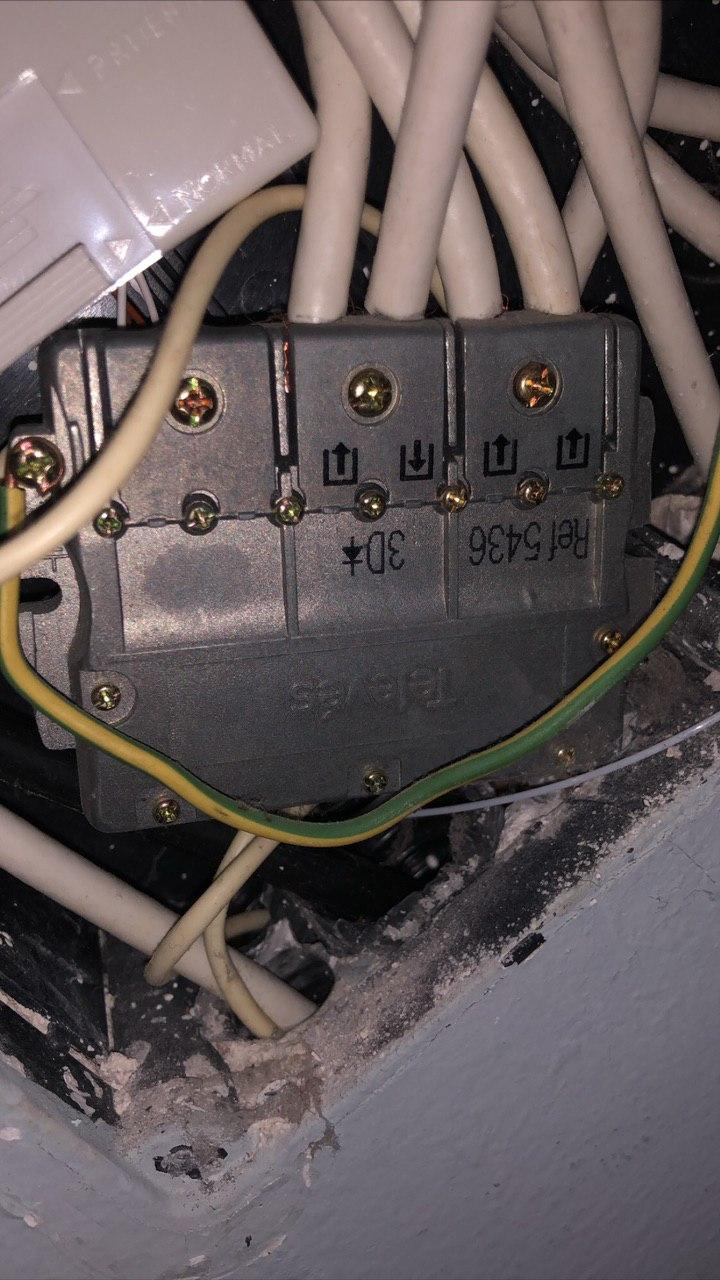
\includegraphics[scale=0.2, angle=-90]{repartidor.jpg}
				\caption{El repartidor $1:3$}
				\label{f:pau}
			\end{figure}

			Como todo equipo emplear una fuente de alimentación no es "gratis" en el sentido de que conllevará una serie de pérdidas que tendremos que contabilizar y que afectarán a todas las tomas del inmueble.\\

		\subsection{Distribución de la red de televisión en el inmueble}
			En el apartado anterior hemos asumido que la vivienda contaba con $4$ tomas sin especificar su localización. Para facilitar el desarrollo de esta sección adjuntamos una fotografía de la planta en la figura \ref{f:p_acotada}. En ella aparecen ligeramente marcadas las estancias de interés así como los lugares aproximados en los que se encuentran las tomas. Si bien es cierto que se muestran las estancias en las que están las tomas no es tan claro dirimir qué son esas estancias. Es por ello que adjuntamos esta información en una pequeña lista:

			\begin{itemize}
				\item \textbf{A} -- Habitación
				\item \textbf{B} -- Cocina
				\item \textbf{C} -- Zona Común
				\item \textbf{D} -- Salón
			\end{itemize}

			\begin{figure}
				\centering
				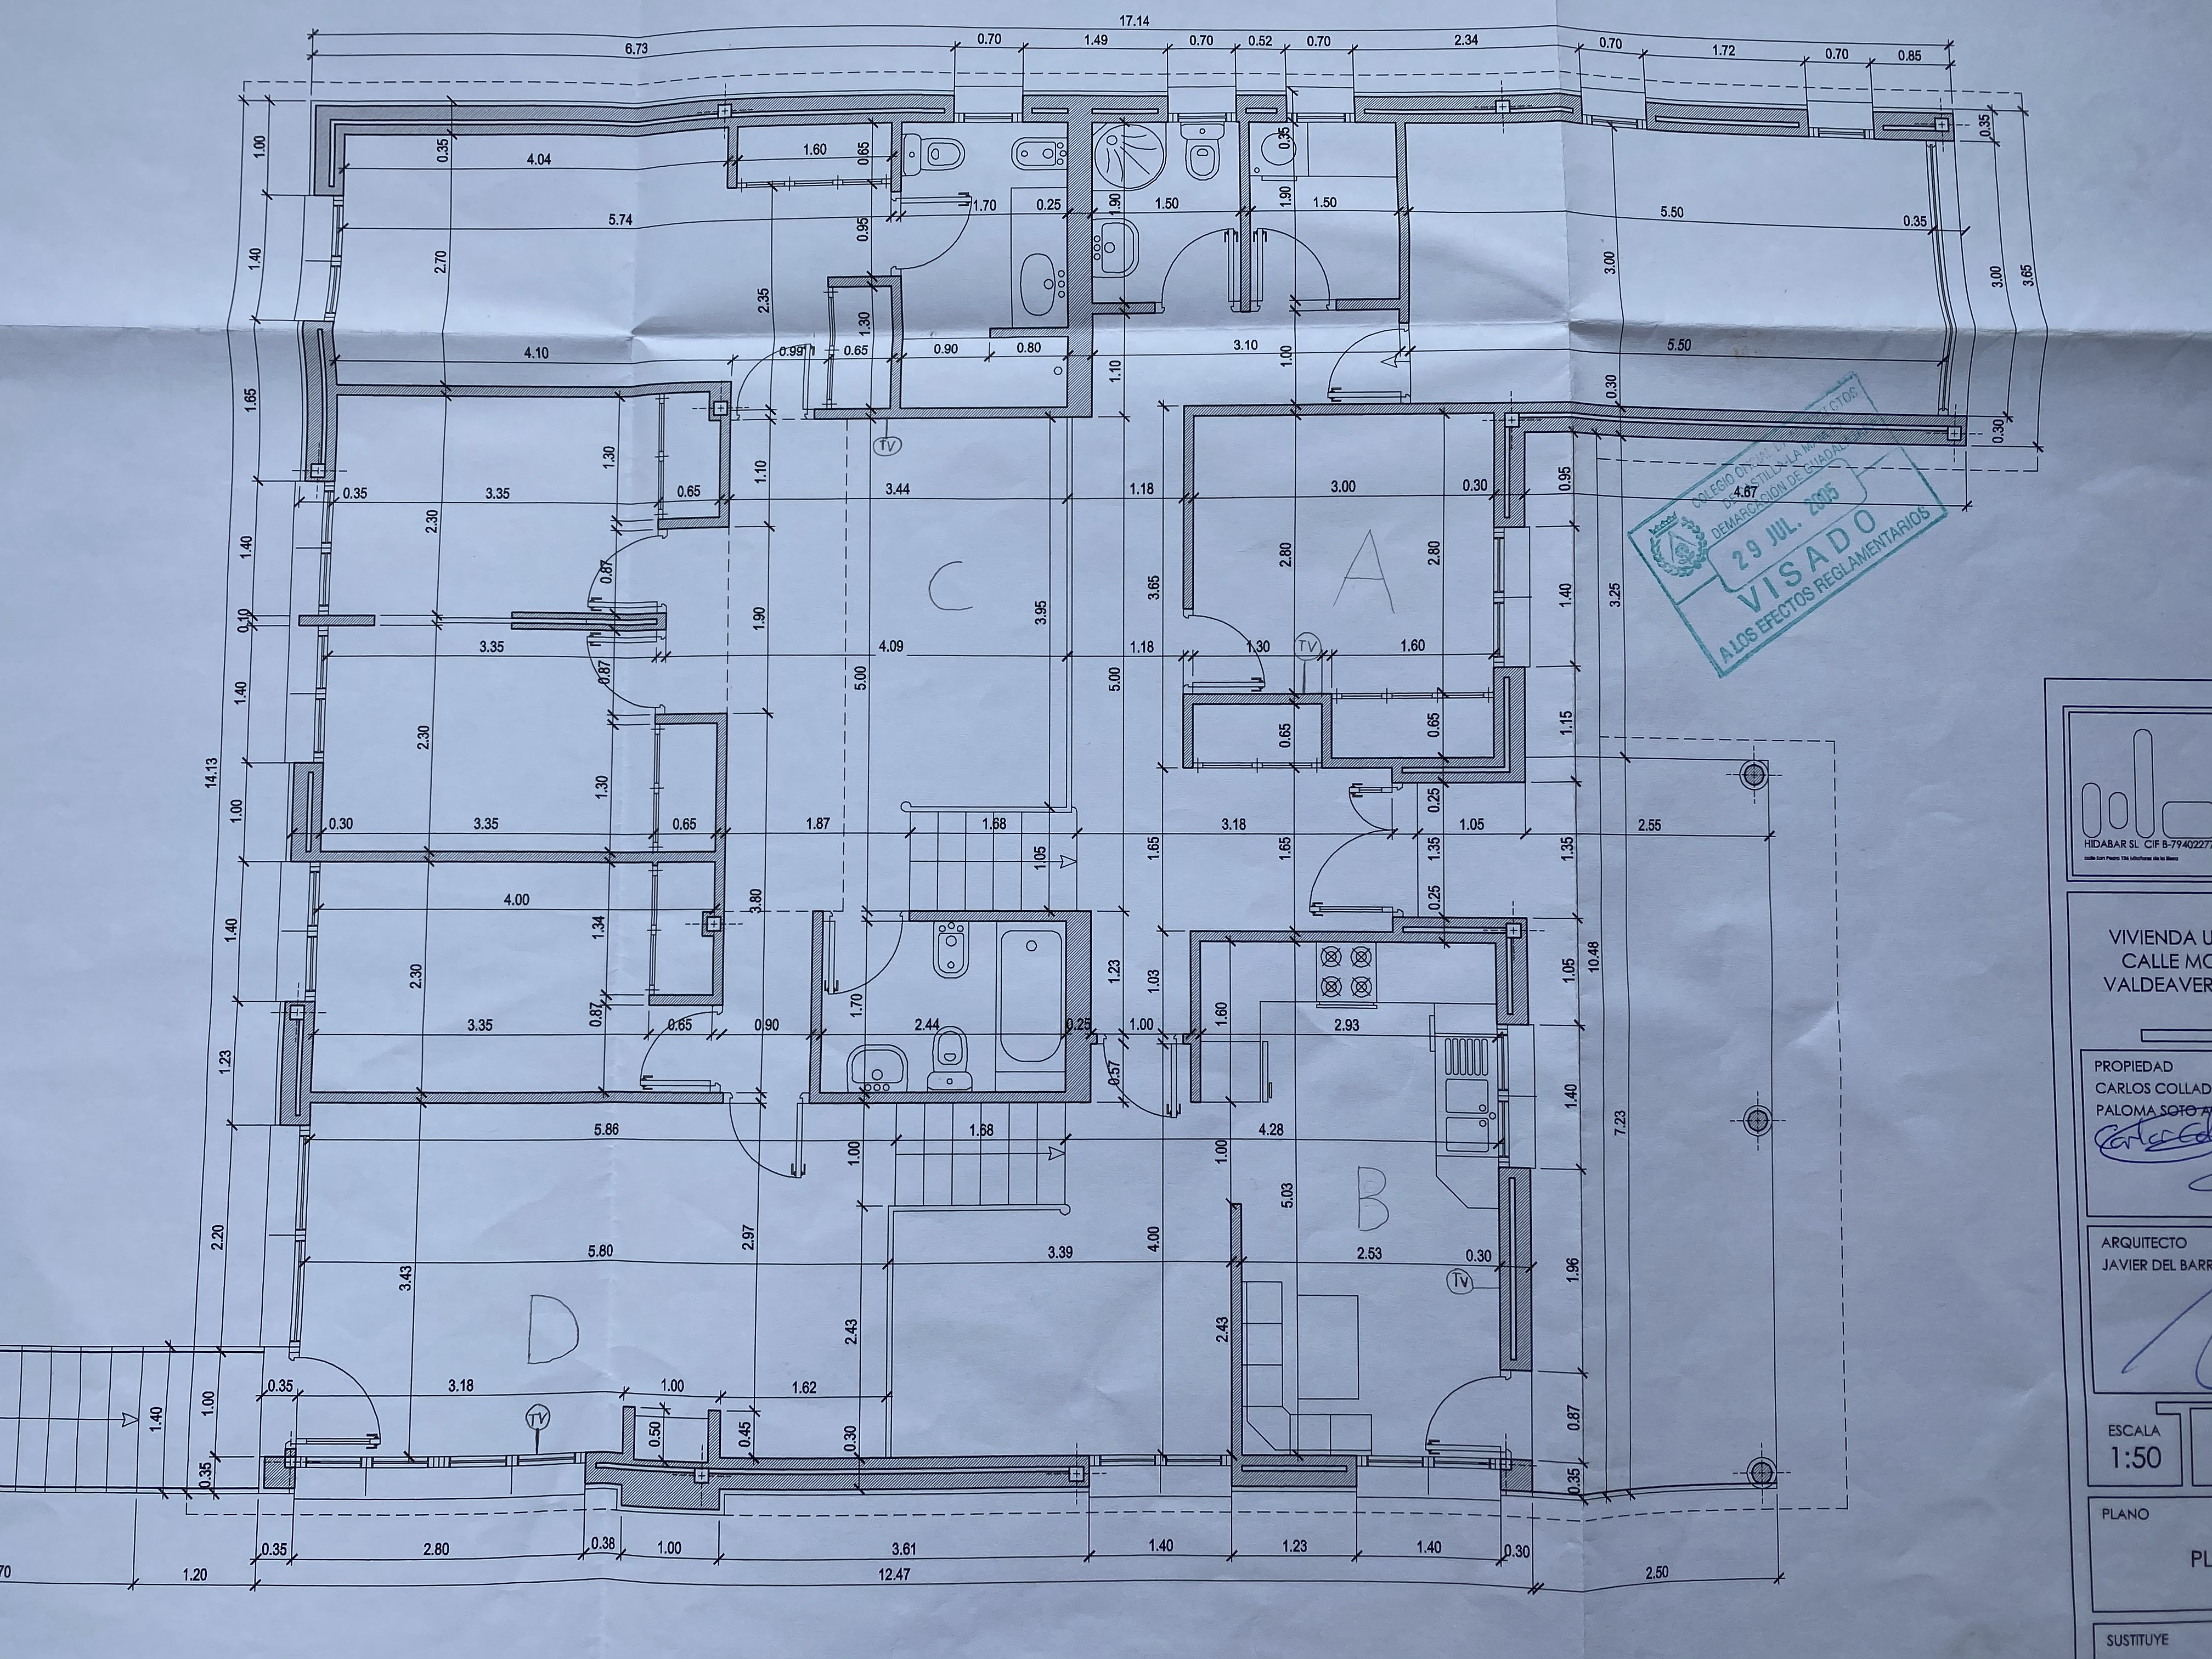
\includegraphics[width=0.8\linewidth]{planta_acotada.jpg}
				\caption{Planta acotada}
				\label{f:p_acotada}
			\end{figure}

			En la imagen que hemos adjuntado también podemos ver las cotas que se han empleado como aproximación de las distancias que emplearemos a la hora de calcular las atenuaciones de la infraestructura.\\

			Señalamos pues que de acuerdo con lo establecido en el \textit{Real Decreto 346/2011 del 11 de marzo} se cumplen los requisitos exigidos. La norma impone que se instalará una toma en cada estancia excluidos baños y trasteros con un mínimo de $2$. Al contar con $4$ tomas estamos alineados con la legalidad.

		\subsection{¿Y el resto de bandas?}
			Hasta ahora solo hemos comentado las características y composición de los equipos de distribución de televisión. No hemos entrado a analizar otras bandas de frecuencia porque la \textbf{ICT} de este edificio \textbf{NO} cuenta con infraestructura capaz de manejar señales satelitales o de audio digital en la \textit{banda III} (\textbf{DAB}). Si cuentan con equipos capaces de captar señales \textbf{FM} en \textit{banda II} pero no son más que pequeñas radios y reproductores \textit{Hi-Fi} con lo que no se engloban dentro del concepto de \textbf{ICT}.\\

			Destacamos además que la operadora que ofrece servicios de telefonía e Internet a la vivienda, \textit{Movistar}, permite instalar una antena parabólica capaz de captar señales satelitales para incluir servicios de televisión de pago. Además de esta antena se debe instalar un decodificador ya que las emisiones se encriptan a fin de que nadie que no posea las claves pertinentes sea capaz de recibir la misma transmisión. A modo de curiosidad comentamos que el antiguo \textit{Canal +} encriptaba las señales de audio y video por separado. La "encriptación" de la primera consistía en invertir el espectro de la señal con lo que era tremendamente sencillo invertirlo de nuevo y obtener el audio de vuelta sin necesidad del equipo de decodificación auxiliar. Dada la linealidad de la definición del espectro de una señal $x(t)$:

			$$X(w) = \int_{-\infty}^{+\infty} x(t) \cdot e^{-jwt}dt \rightarrow -X(w) = \int_{-\infty}^{+\infty} -x(t) \cdot e^{-jwt}dt \rightarrow \mathcal{F}^{-1}\{-X(w)\} = -x(t)$$

			Observamos que si se invierte el espectro la señal que recuperamos está invertida. Si aplicamos un inversor, una configuración muy típica con amplificadores operacionales, podemos recuperar esta señal sin ningún tipo de problema.

		\subsection{Red Telefónica y de Datos}
			Ya en la introducción habíamos señalado que el acceso telefónico y de datos del inmueble estudiado se sustentaba sobre una línea ADSL. Esta conexión se compone de un par trenzado de cobre que une el punto de terminación de red de cada vivienda con el \textbf{DSLAM} del operador. Este \textbf{DSLAM} "traduce" las señales analógicas del cable de cobre a señalización digital que luego se cursará por Internet. Si prestamos atención a la red telefónica veremos que la señal de voz es posteriormente desviada a la red orientada a circuitos que cursa el tráfico de voz. En definitiva aunque el tráfico de voz y datos se curse por los enlaces de cobre debemos saber que este luego se separa en función de su naturaleza.\\

			Nos podemos preguntar ahora cómo es posible que 2 tráficos totalmente distintos convivan en un solo conductor. La respuesta está en el dominio de la frecuencia. La señal que viaja por el cable sería:

			$$x(t) = x_{voz}(t) + x_{datos}(t)$$

			Si analizamos $X(w) = \mathcal{F}\{x(t)\}$ nos daremos cuenta de que:

			$$X(w) = X_{voz}(w) + X_{datos}(w)$$

			Y lo que es más:

			$$X_{voz}(w) = 0\ \forall \ w \ \notin [0, 14]\ kHz;\ X_{datos} = 0\ \forall w \in [0, 14]\ kHz$$

			En definitiva, los espectros de ambos tipos de señales no se superponen por lo que filtrando alrededor de $14\ kHz$ podemos separar ambas señales sin ningún tipo de problema. Este filtrado es lo que está haciendo el \textit{splitter} que mencionábamos antes. Así es como conseguimos explicar que tanto el "router" como el teléfono fijo estén conectados en última instancia a la misma toma de pared. El splitter no es más que un filtro paso bajo que extrae la señal de voz de la superposición que existe en el cable.\\

			\begin{figure}
				\centering
				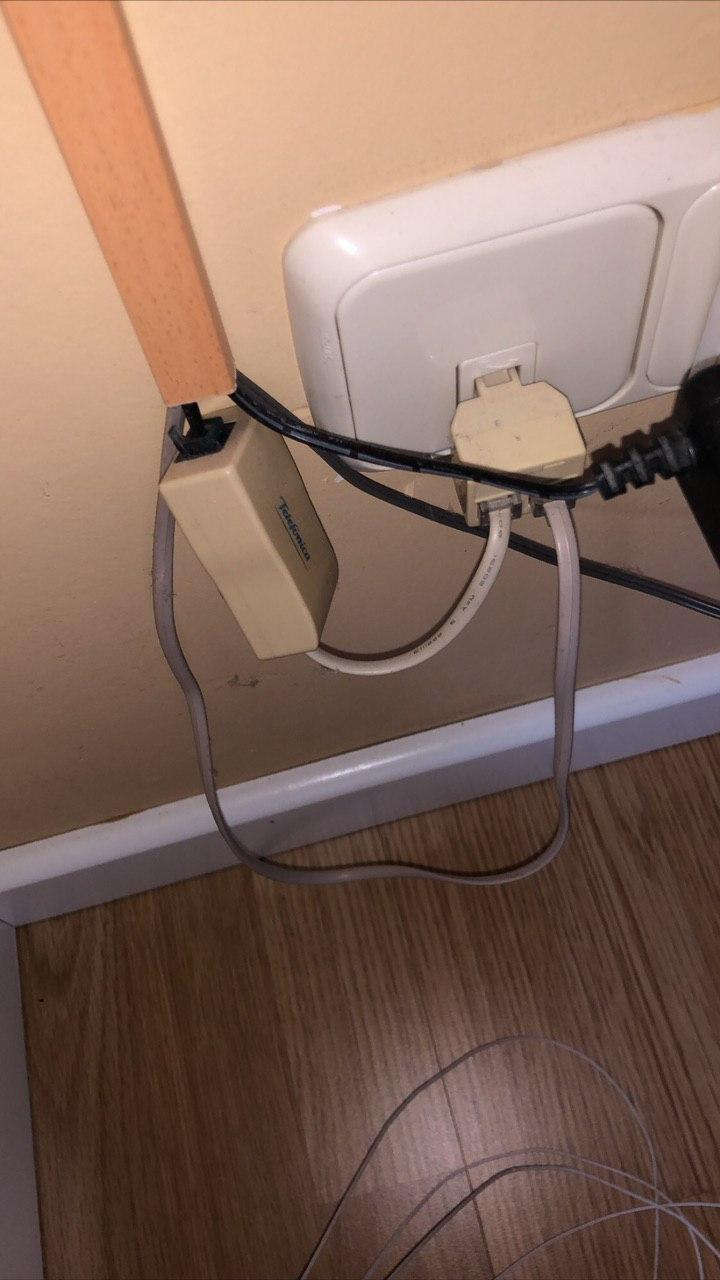
\includegraphics[scale=0.2]{splitter.jpg}
				\caption{Splitter}
				\label{f:splitter}
			\end{figure}

			\begin{figure}
				\centering
				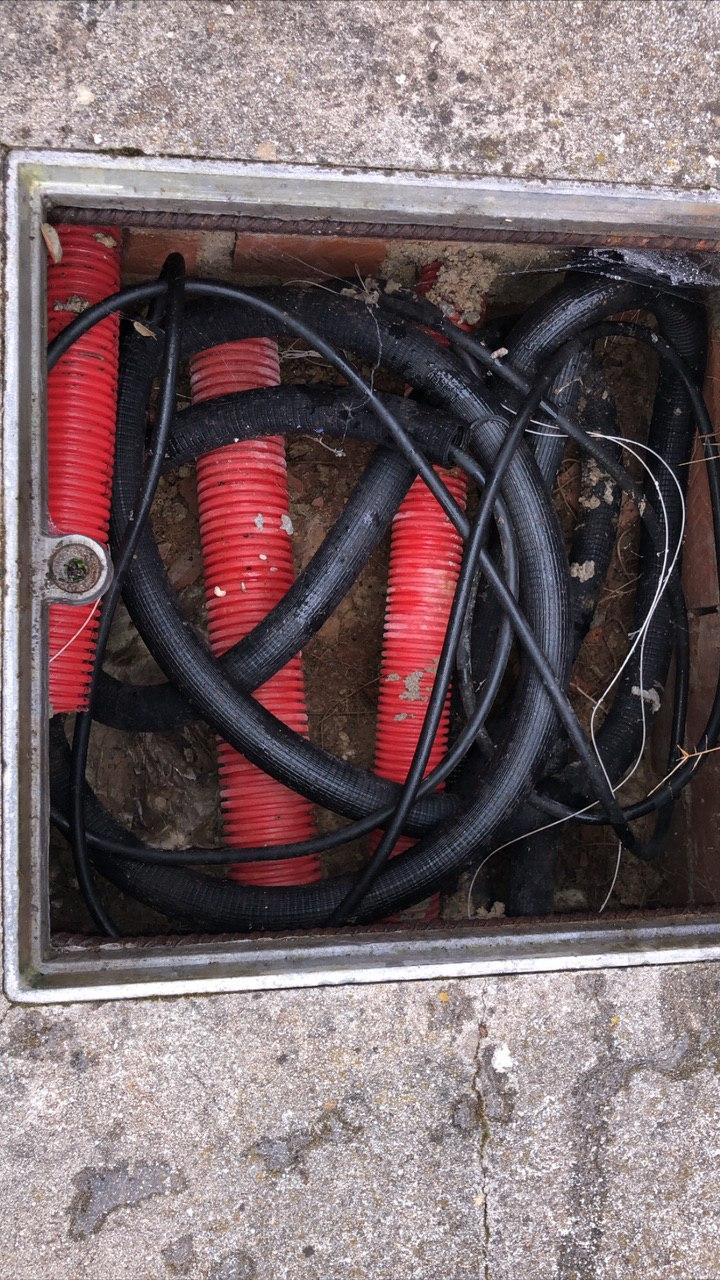
\includegraphics[scale=0.3, angle=90]{arqueta.jpg}
				\caption{Arqueta del jardín}
				\label{f:arqueta}
			\end{figure}

			Al referirnos anteriormente al router lo hemos entrecomillado porque en el aparato que nos da la operadora tenemos tanto un encaminador de capa 3 (un router tradicional) como un módem que adapta los paquetes de información con un formato digital a señales de naturaleza analógica. Además también contará con el filtro paso-alto pertinente.\\

			El punto de terminación de red se encuentra en el registro primario junto al equipo de televisión digital terrestre y marca el límite entre la red del operador y la del abonado. Permite "pinchar" un terminal en ese punto de la línea para comprobar si los errores de red se localizan en la red del abonado o en la externa. Atendiendo a esta definición la línea de cobre (en negro) que se encuentra en la arqueta de la figura \ref{f:arqueta} es todavía parte de la red del operador.\\

			Con todo esperamos haber esclarecido aunque sea ligeramente la anatomía de las redes ADSL.

	\newpage

	\section{Cálculos realizados}
		\subsection{Atenuaciones}
			Para llevar a cabo los cálculos de las pérdidas producidas en toda la instalación desplegada a lo largo de la vivienda así como su posterior comprobación mediante la herramienta de simulación de la que disponemos hemos debido tener en cuenta una serie de consideraciones. Por una parte, hemos llevado a cabo una aproximación de todas las mediciones y distancias pues en los planos proporcionados con anterioridad por el arquitecto encargado de todo el diseño del tendido para televisión no se explicitaba el recorrido seguido por los cables desde el registro primario hasta cada una de las cuatro tomas de televisión existentes en el inmueble, empleando para ello las distancias y mediciones apreciables a través del pertinente estudio de la planta acotada.\\

			De forma similar, la correspondiente verificación con el programa \textit{Cast 60} nos ha presentado ciertas dificultades pues algunos de los componentes presentes en nuestra entramado real no presentan su equivalente en la simulación, siendo esto una gran limitación para corroborar la fidelidad de los cálculos.\\

			Tal y como comentábamos con anterioridad disponíamos de una fuente de alimentación que además de llevar a cabo su cometido requerido se encargaba de establecer una conexión directa con una de las tomas existentes. He aquí donde, debido a las dificultades ya citadas previamente, hemos tenido que realizar una serie de suposiciones, como es el caso de cuál de las 4 terminaciones es alcanzada por la salida de la fuente de alimentación. Así, hemos considerado que se trata de la que se encuentra más próxima al registro primario, es decir, a una menor distancia.\\

			Las mediciones obtenidas tras el estudio de la planta acotada necesarias para nuestro análisis son:

			\vskip 3mm

			\begin{center}
				\begin{tabular}{| c | c | c |}
					\hline
					\textbf{Distancias} & \textbf{Valor} & \textbf{Unidad}\\
					\hline
					Antena a amplificador & 1 & m\\
					\hline
					Amplificador a fuente de alimentación & 3 & m\\
					\hline
					Fuente de alimentación a PAU & 0.5 & m\\
					\hline
					Fuente de alimentación a toma 1 & 5,25 & m\\
					\hline
					PAU a toma 2 & 6,423 & m\\
					\hline
					PAU a toma 3 & 11,752 & m\\
					\hline
					PAU a toma 4  & 19,805 & m\\
					\hline
				\end{tabular}
			\end{center}

			\vskip 3mm

			Para realizar los cálculos correspondiente hemos echado mano del catálogo de dispositivos de Televés disponible en el aula virtual de la asignatura así como de la propia página web de la mencionada compañía para el caso de aquellos elementos no presentes en el referido folleto.\\

			De este modo, la información de nuestro interés obtenida es:

			\vskip 3mm
			\begin{center}
				\begin{tabular}{| c | c | c |}
					\hline
					\textbf{Elemento} & \textbf{Valor} & \textbf{Unidad}\\
					\hline
					Pérdidas de inserción fuente de alimentación (5495) & 4 & dB\\
					\hline
					Pérdidas de inserción PAU (5436) & 7 & dB\\
					\hline
					Pérdidas cable (2138) & 0.18 & dB/m @ 800 MHz\\
					\hline
					Pérdidas cable (2141) & 0.15 & dB/m @ 800 MHz\\
					\hline
					Pérdidas derivación toma (5226) & 0.6 & dB\\
					\hline
					Ganancia amplificador (5356) & 40 - [0, 15] & dB\\
					\hline
					Figura de ruido del amplificador (5356) & 5.5 & dB\\
					\hline
				\end{tabular}
			\end{center}

			\vskip 3mm

			Tras haber realizado los pertinentes cálculos en cuanto a las pérdidas de toda la instalación, sumando las presentadas por los cables, los dispositivos intermedios como la fuente de alimentación y el punto de acceso de usuario y las restantes tomas de televisión, hemos apreciado una considerable diferencia entre aquella terminación que establece una unión directa con la fuente de alimentación y las que deben pasar previamente por la PAU.\\

			Para evidenciar más esta variación presentamos los cálculos para todos los casos, teniendo en cuenta las mediciones y parámetros presentados con anterioridad:

			\begin{multline*}
				$$L(dB)_{toma1} = 4\ m\ \cdot\ 0.18\ \frac{dB}{m}\ +\ 4\ dB\ +\ 0\ dB\ +\ 0\ dB\ +\ 5.25\ m\ \cdot\\
				\cdot 0.15\ \frac{dB}{m}\ +\ 0.6\ = 6.1075\ dB$$
			\end{multline*}

			\begin{multline*}
				$$L(dB)_{toma2} = 4\ m\ \cdot\ 0.18\ \frac{dB}{m}\ +\ 4\ dB\ +\ 0.5\ m\ \cdot\ 0.15\ \frac{dB}{m}\ +\\
				+ 7\ dB\ +\ 6.423\ m\ \cdot\ 0.15\ \frac{dB}{m}\ +\ 0.6\ dB = 13.35845\ dB$$
			\end{multline*}

			\begin{multline*}
				$$L(dB)_{toma3} = 4\ m\ \cdot\ 0.18\ \frac{dB}{m}\ +\ 4\ dB\ +\ 0.5\ m\ \cdot\ 0.15\ \frac{dB}{m}\ +\\
				+ 7\ dB\ +\ 11,752\ m\ \cdot\ 0.15\ \frac{dB}{m}\ +\ 0.6\ dB = 14.1578\ dB$$
			\end{multline*}

			\begin{multline*}
				$$L(dB)_{toma4} = 4\ m\ \cdot\ 0.18\ \frac{dB}{m}\ +\ 4\ dB\ +\ 0.5\ m\ \cdot\ 0.15\ \frac{dB}{m}\ +\\
				+ 7\ dB\ +\ 19.805\ m\ \cdot\ 0.15\ \frac{dB}{m}\ +\ 0.6\ dB = 15.36575\ dB$$
			\end{multline*}

			Si queremos ser estrictos debemos calcular estas atenuaciones en dos frecuencias significativas dentro de la región \textbf{UHF} en la que estmos trabajando. Ya en la introducción comentábamos que la region anterior comprendía $2$ bandas: \textit{BIV} y \textit{BV}. Tal y como se observa tenemos $2$ fuentes principales de atenuación. Por un lado los cables coaxiales atentan contra la señal de manera proporcional a su longitud. Observamos después que los repartidores tienen también una incidencia negativa sobre la integridad del nivel deseado.\\

			Además nos gustaría comentar un poco la extraña decisión de diseño que se ha llevado a cabo. Observamos cómo la \texttt{toma 1} que es la más cercana al registro no sufre las pérdidas de inserción de la \texttt{PAU}. Lo "normal" sería que la toma que no conectamos a través de este aparato sea la que más alejada está del registro en un intento de equilibrar las atenuaciones. No obstante y juzgando por la dirección de los coaxiales al entrar en el tabique la instalación parecía ser la que hemos descrito. Al no poder levantar el suelo para observar el recorrido de estos cables nos debemos conformar con nuestra intuición... Esto suscita un aspecto que a veces nos pasa desapercibido y es que por mucho que la ley dictamine una serie de protocolos muchas veces estos no se siguen al pie de la letra en instalaciones reales. Nos puede interesar más que una instalación sea sencilla que que cumpla con la normativa de manera estricta siempre y cuando se mantengan unos mínimos como son los niveles de señal en las tomas. Simplemente queríamos comentar este aspecto ya que, tal y como decíamos, muchas veces no somos conscientes de lo diferentes que pueden llegar a ser los escenarios teóricos y los reales.\\

			Sabemos que las pérdidas son una función de la frecuencia. Al estar analizando un rango y no una frecuencia puntual podríamos pensar que estas atenuaciones variarán en función de qué referencia tomemos. Si bien esto es cierto los catálogos suelen ofrecer la atenuación de sus equipos para rangos de frecuencias como el de la televisión digital con lo que estas pérdidas serán contantes en toda la ragión \textbf{UHF}. Lo mismo no es cierto para los coaxiles, aprecuando como cabría esperar una mayor atenuación a medida que incrementa la frecuencia. Es por esto que especificábamos que las atenuaciones se daban para una frecuencia de $800\ MHz$. Si bien este no es el límite estricto de la \textit{BV} es el que se asume al analizar este tipo de instalaciones. Podríamos haber escogido la atenuación a $500\ MHz$ ya que también se incluye en el rango de interés pero estaríamos cometiendo un error ya que no estaríamos trabajando con el peor caso posible y por tanto corremos el riesgo de infradimensionar nuestro sistema.\\

			Debemos señalar que tal y como habíamos comentado los valores que estamos empleando son los del catálogo facilitado en la web de la asignatura. Hemos querido cerciorarnos de que estos valores son correctos y es por ello que hemos tratado de obtener lo mismo empleando el programa de diseño de \textbf{ICT}s \textit{Cast 60}. Las medidas que hemos obtenido en esta herramienta son coherentes con las derivadas a partir del catálogo pero no exactamente iguales. Los valores internos que emplea este programa son a veces ligeramente distintos de los que se proporcionan en otras fuentes y debemos tolerarlos ya que las características de sus componentes no se pueden alterar. Más delante incluimos una tabla con estos valores en los que se observan estas ligeras desviaciones.\\

			Emplear este software también ha supuesto tener que en cierto modo corregir la inexistencia de la fuente de alimentación entre sus componentes. Para tratar de ser lo más veraces posible hemos sustituido este elemento por uno repartidor de dos tomas con una pérdida de inserción análogas a las de esta fuente. Para ello consultamos las especificaciones del equpio \textit{5495} que son $4\ dB$ tal y como comentábamos para en su lugar emplear el repartidor \textit{5150} con unas similares. Es por ello que en el esquema que se observa en la figura \ref{f:cast60} aparece este elemento.\\

			\begin{figure}
				\centering
				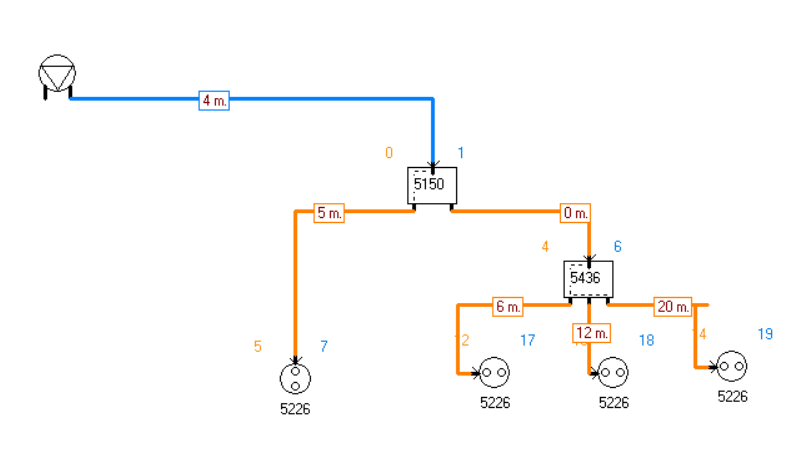
\includegraphics[scale=0.8]{esquema_mitad.png}
				\caption{Esquema de la instalación en \textit{Cast 60}}
				\label{f:cast60}
			\end{figure}

			Gracias a esta herramienta hemos obtenido estas atenuaciones teniendo en cuenta una frecuencia de $500\ MHz$ y hemos adjuntado estas nuevas medidas así como las proporcionadas por \textit{Cast 60} para $800\ MHz$ en una tabla que facilita su comparación. Hemos decidido no incluir los cálculos detallados de estos últimos valores porque son totalmente análogos a los anteriores teniendo en cuenta las siguientes atenuaciones de los coaxiales:

			\begin{itemize}
				\item Coaxial 2138 -- 14 dB/m @ 500 MHz
				\item Coaxial 2142 -- 12 dB/m @ 500 MHz
			\end{itemize}

			Con esto, llegamos a los siguientes resultados para las atenuaciones en toma:

			\begin{center}
				\begin{tabular}{| c | c | c |}
					\hline
					& Atenuación \textit{BIV} $[dB]$ & Atenuación \textit{BV} $[dB]$\\
					\hline
					Toma 1 & 5.97 & 6.13\\
					\hline
					Toma 2 & 13.2 & 13.39\\
					\hline
					Toma 3 & 13.96 & 14.21\\
					\hline
					Toma 4 & 14.6 & 14.95\\
					\hline
				\end{tabular}
			\end{center}

			Si bien se observa una ligera desviación en medidas coma la de la tercera toma donde comparamos los $14.21\ dB$ de \textit{Cast 60} con los $14.1578\ dB$ obtenidos teóricamente suponiendo esto un error de apenas $5$ centésimas que supone un factor de $1.012$ en unidades lineales. Esta magnitud se sigue de la definición misma de las unidades logarítmicas:

			$$5 \cdot 10^{-2} = 10 \cdot log(\frac{L_{soft}}{L_{theo}}) \rightarrow \frac{L_{soft}}{L_{theo}} = 10^{5 \cdot 10^{-3}} \approx 1.012$$

			Nos queda señalar por último que a la hora de emplear el repartidor \textit{5436} hemos encontrado que una de las salidas presentaba una atenuación de medio $dB$ menos que las demás. El catálogo de la asignatura no contempla este comportamiento pero para nuestra sorpresa el modelo actual del aparato \textbf{SÍ} muestra una atenuación distinta en función de las salidas. Nosotros hemos asumido una atenuación uniforme pero si se usa este nuevo modelo emplearíamos la salida con una menor atenuación para la toma más lejana en un intento de suavizar las diferencias de nivel entre una y otra.\\

			Con las atenuaciones claras pasamos a comprobar si este nivel es aceptable para una instalación conforme a las normas establecidas.

		\subsection{Niveles en toma y amplificación de la entrada}
			A la luz de todo el diseño solo nos queda comentar las características de nuestro amplificiador de cabecera. Teniendo en cuenta que la ley establece un nivel en el rango de los $[47,\ 70]\ dB\mu V$ en toma debemos averiguar nuestra mínima atenuación para poder diseñar contra ese límite. Así, tal y como comentábamos la menor atenuación será de $5,97\ dB$ en la \texttt{toma 1} para la \textit{BIV} tal y como se obtiene del programa \textit{Cast60}. Aplicando la siguiente expresión:

			$$V_{amp}(dB\mu V) = 70 dB\mu V + L_{min}(dB)$$

			Observamos que la salida del amplificador debería ser $V_{amp}(db\mu V) = 75,97\ dB\mu V$. Este nivel es el máximo admisible para nuestra instalación con lo que nos aseguramos de que los niveles sigan siendo válidos aún en las tomas que sufren una mayor atenuación.\\

			Según los catálogos, la ganancia de nuestro amplificador de cabecera (el modelo $5356$) es de $40\ dB$. No obstante tenemos una atenuación regulable de hasta $15\ dB$ lo que supone que la ganancia de nuestro amplificador va a encontrarse en el rango: $G \in [25,\ 40]\ dB$. Donde $25 = 40 - 15$, es decir, sería el factor de amplificación con la mayor atenuación posible. Con esto en mente, nuestra señal de entrada oscilará entre los valores que vienen definidos por las siguientes expresiones:

			$$V_{in_{MAX}} = V_{amp_{MAX}} - G_{min} = 75,97\ dB\mu V - 25\ dB = 50,97\ dB\mu V$$
			$$V_{in_{min}} = V_{amp_{MAX}} - G_{MAX} = 75,97\ dB\mu V - 40\ dB = 35,97\ dB\mu V$$

			En otras palabras, la señal a la entrada (esto es, la captada por la antena) pertenecerá al intervalo $V_{in} \in [35,97,\ 50,97]\ dB\mu V$. Sin tener acceso a la antena ni al equipo especializado que se requiere para medir estos niveles todo lo que podemos hacer es obtener el rango de niveles que puede presentar la señal a la entrada... A la hora de instalar esta infraestructura los técnicos seguramente variarían la atenuación hasta que la señal de \texttt{TV} se viera correctamente en la propia televisión.\\

			Con todo, observamos cómo el programa \textit{Cast 60} valida la \textbf{ICT} que aparece en la figura \ref{f:cast60}.\\

			Atendiendo a la figura de ruido del amplificador asistimos pues a una relación señal ruido ($SNR$) de:

			$$SNR = 60\ dB\mu V - 5.5\ dB - 2.8\ dB = 51.7\ dB$$

			% \textbf{NOTA: Creemos que el $2.8\ dB$ se relaciona con el ruido aditivo Gaussiano del canal. ¿Es eso cierto?}

			Finalmente incluimos una imagen en la que se aprecia el amplificador de cabecera conectado al mástil de nuestra antena en la figura \ref{f:amp_cabecera}.

			\begin{figure}[hbt!]
				\centering
				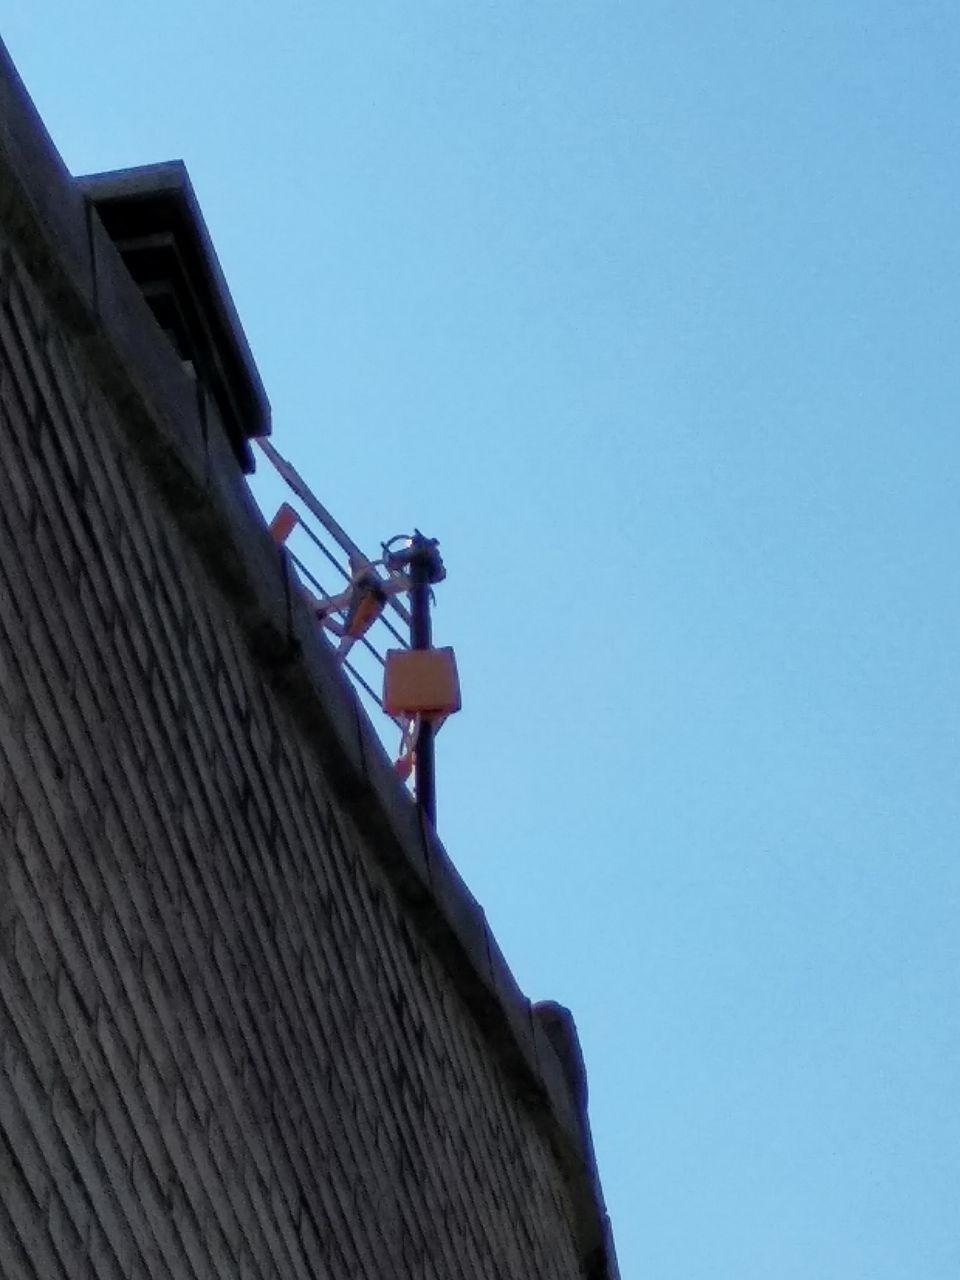
\includegraphics[width=0.5\linewidth]{amp_cabecera.jpg}
				\caption{Amplificador de cabecera (en naranja)}
				\label{f:amp_cabecera}
			\end{figure}

	\section{Conclusión}
		A lo largo de este informe hemos recorrido la anatomía de las infraestructuras de telecomunicación típica de las viviendas unifamiliares. Esto nos ha servido no solo para ahondar en los conceptos vistos en clase sino también para obsevar cómo conviven las infraestructuras de datos, voz y televisión así como lo sencillas que resultan estas instalaciones en comparación con las estudiadas para bloques de pisos.\\

		Esperamos haber aportado un toque original a este tema a través del análisis del tipo menos común de \textbf{ICT} que no por ello supone un menor reto ni un menor número de aspectos interesantes. Esperamos haber sido capaces de captar estos detalles a la vez que excavábamos un poco más en la dimensión más teórica de este tema como puede ser el dominio frecuencial y la definición y manejo de las unidades logarítmicas.\\
\end{document}
